\chapter{Implicit ODE solver}
In the following, we consider the initial value problem (IVP) on the form
\begin{align}
    \dot{x}(t) &= f(t,x(t),p), & x(t_0) = x_0,
\end{align}
where $x \in \probR ^{n_x}$ and $p \in \probR ^{n_p}$. 

\section{Description of implicit Euler}
Our goal is to solve the IVP using a scientific, i.e., numeric, method. We note that $\dot{x}(t+h)$ is given by the limit (multiple equal limits exist)
\begin{align}
    \lim_{h \rightarrow 0} \dot{x}(t+h) &:= \lim_{h \rightarrow 0} \frac{x(t+h)-x(t)}{h}.
\end{align}
Since we are using numerical methods, we cannot represent the actual limit value. Instead, we have to use some finite approximation thereof. Choosing some $h>0$ therefore naturally leads to the approximation
\begin{align}
    \dot{x}(t+h) &\approx \frac{x(t+h)-x(t)}{h}, &h>0.
\end{align}
By rearranging the terms (isolating $x(t+h)$) we get
\begin{align}
    x(t+h) \approx x(t+h) + \dot{x}(t) h.
\end{align}
In fact, this corresponds to a first order Taylor expansion. From our basic course in calculus we therefore know that
\begin{align}
    x(t+h) &= x(t) + \dot{x}(t+h) h + \mathcal{O}(h^2).
    \label{eq3:im_euler}
\end{align}
This method is known as the implicit Euler method. Notice that unlike the explicit Euler method we do not know all terms on the right hand side. In stead, we must solve the equation
\begin{align}
    x(t+h) - (x(t) + \dot{x}(t+h) h) &= 0.
\end{align}
This is usually done using e.g. Newton's method. However, since it is only an approximation, we might as well loosen the restriction a bit, and consider 
\begin{align}
    x(t+h) - (x(t) + \dot{x}(t+h) h) &\leq \varepsilon, & \varepsilon>0.
\end{align}
This is known as \textit{in-exact Newton} and might produce a significant increase in speed for the method. 

We now have an alternative way of estimating $x(t+h)$. The implicit Euler method is more stable for stiff problems, i.e., problems with rapidly changing dynamics. Since an equation must be solved for each step, the steps are generally more expensive than for the explicit Euler method, so the implicit method must only be used when needed. If we compare the stability regions of the test equation for the explicit and implicit methods, we see that the implicit Euler method has a much larger stability region than the explicit Euler method. So much so that the implicit Euler method might converge even when the problem is actually not stable! 

\section{Implicit Euler fixed time step implementation}
When using the implicit Euler method, it is important to choose a suitable step size, $h$. Figure \ref{fig1:im_stability} shows the stability region of the implicit Euler method for $\mu = \lambda h$ for the test equation. Notice that \textit{suitable} has to be seen in the in the context of the problem at hand. The most simple approach is to use a fixed step size; however, when doing so the user must select it very carefully. Listing \ref{lst3:im_euler} shows a Matlab implementation of the implicit Euler method.

\begin{lstlisting}[language=Matlab,caption=Implicit Euler with fixed step size.,label=lst3:im_euler]
function [t,x,count_f] = ImplicitEuler(fun,ta,tb,n,xa,varargin)
    % Implicit euler scheme
    % f(x_t+1) = f(x_t) + f'(x_t+1)*h
    
    h = (tb-ta)/n;
    nx = size(xa,1);
    x = zeros(nx,n+1);
    t = zeros(1,n+1);
    count_f = 0; 

    tol = 1.0e-6;
    maxit = 100;

    t(:,1) = ta;
    x(:,1) = xa;
    for k=1:n
        [f,~] = feval(fun,t(k),x(:,k),varargin{:});
        t(:,k+1) = t(:,k) + h;
        x0 = x(:,k) + h*f;
        [x(:,k+1),count,~] = NewtonsMethodODE(fun,t(:,k), x(:,k), h, x0, tol, maxit,varargin{:});
        count_f = count_f + count;
    end

    t = t';
    x = x';

    end
\end{lstlisting}

\section{Implicit Euler adaptive time step implementation}
Sometimes it can be difficult to select a suitable step size, $h$. When dealing with problem with a more rich dynamic than the test equation, we might see that a smaller step size might be required in parts of the solution than others. To overcome this problem with a fixed step size, we must select a small step size and use that everywhere. However, this comes with a significant penalty to the speed, since we could get away with using a larger step size in most of the solution. This problem leads to a natural desire to construct an algorithm that can change the step size adaptively. The goal is to use as large step size as possible, while maintaining a sufficient accuracy in the individual steps. 

We therefore need some way of estimating the error, we do so using what is known as \textit{step doubling}. We have
\begin{align}
    x_{k+1} &= x_k + hf(t_k,x_k), \\
    \hat{x}_{k+1/2} &= x_k + \frac{h}{2}f(t_k,x_k), \ \text{and} \\
    \hat{x}_{k} &= \hat{x}_{k+1/2} + \frac{h}{2}f(t_k+\frac{h}{2},\hat{x}_{k+1/2}).
\end{align}
We now get the error estimate by means of step doubling by
\begin{align}
    e_{k+1} &= \hat{x}_{k+1} - x_{k+1}.
\end{align}
We are now able to define how to select the best step size, $h$. We do so by the \textit{asymptotic step size controller}, this means that our step size is given by
\begin{align}
    h_{k+1} &= \left(\frac{\varepsilon}{r_{k+1}} \right )^{1/2} h_k.
\end{align}
Where $r_{k+1}$ is found by
\begin{align}
    r_{k+1} &= \max_{i \in \{1,...,n_x\}} \left \{ \frac{|e_{k+1}|_i}{ \max \{ |\text{abstol}|_i, \ |x_{k+1}|_i \cdot |\text{reltol}|_i \} } \right \}
\end{align}
where $|\text{abstol}|_i$ and $|\text{reltol}|_i$ are the absolute and relative tolerance of $(x_{k+1})_i$ respectively. Listing \ref{lst3:im_euler_adap} shows a matlab implementation of implicit Euler method with step doubling and asymptotic step size controller. 

\begin{lstlisting}[language=Matlab,caption=Implicit Euler with adaptive step size.,label=lst3:im_euler_adap]
function [T,X,E,R,H,count_nfun,count_acp,count_rej] = ImplicitEulerAdaptiveStep(fun,tspan,x0,h0,abstol,reltol,varargin)
    % Implicit euler scheme with adaptive step length (h)
    % f(x_t+1) = f(x_t) + f'(x_t+1)*h
    
    epstol = 0.8; 
    facmin = 0.1; 
    facmax = 5.0; 

    t0 = tspan(1); 
    tf = tspan(2); 

    t = t0; 
    h = h0; 
    x = x0; 

    T = t; 
    X = x'; 
    E = 0;
    R = 0;
    H = h0; 
    
    count_acp = 0; 
    count_step = 0; 
    count_nfun = 0; 
    count_rej = 0; 

    while t < tf 
        if (t+h>tf)
            h = tf - t; 
        end 

        f = feval(fun,t,x,varargin{:});
        AcceptStep = false;
        while ~AcceptStep
            x0 = x + h*f; 
            [x1,count1,~] = NewtonsMethodODE(fun,t, x, h, x0, tol, maxit,varargin{:});

            hm = 0.5*h; 
            tm = t + hm; 
            x0 = x + hm*f; 
            [xm,count2,~] = NewtonsMethodODE(fun,t, x, hm, x0, tol, maxit,varargin{:});

            fm = feval(fun,tm,xm,varargin{:});
            x0 = xm + hm*fm; 
            [x1hat,count3,~] = NewtonsMethodODE(fun,tm, xm, hm, x0, tol, maxit,varargin{:});

            e = x1hat-x1; 
            r = max( abs(e) ./ max(abstol, abs(x1hat).*reltol) ); 

            AcceptStep = (r <= 1.0);
            if AcceptStep
                t = t+h; 
                x = x1hat; 
                E = [E;abs(e)'];
                R = [R;r];
                H = [H;h];

                T = [T;t];
                X = [X;x'];
                count_acp = count_acp + 1;
            else 
                count_rej = count_rej + 1; 
            end
            h = max(facmin, min(sqrt(epstol/r),facmax))*h; % change step size
            count_step = count_step + 1;
            count_nfun = count_nfun + count1 + count2 + count3;
        end 
        count_nfun = count_nfun + count_step + count_rej;
    end 
\end{lstlisting}

\section{Test on Van der Pol problem and comparison with Matlab ODE solvers}
Now that we have made an implementation of the implicit Euler method with both fixed and adaptive step size we want to compare these. To do so we look at the Van der Pol problem given by
\begin{align}
    \Ddot{x}(t) &= \mu (1-x(t)^2) \dot{x}(t) - x(t).
\end{align}
To solve the problem using the implicit Euler method we must first re-write the problem as a system of first order differential equations. Luckily this is done easily and given by
\begin{align}
    \dot{x}_1(t) &= x_2(t) \\
    \dot{x}_2(t) &= \mu(1-x_1(t)^2) x_2(t) - x_1(t).
\end{align}

We will now test the implicit Euler method on the Van der Pol problem with $\mu = 3$ and $\mu = 20$. 

\subsection{Van der Pol, $\mu = 3$}
The Van der Pol problem with $\mu = 3$ is a relatively straight forward non-stiff problem. There is no formal definition of when a problem is \textit{stiff}---only that whenever a problem change dynamics "very quickly" it is said to be. 

Figure \ref{fig3:fixed_mu3} shows the numerical solution to the Van der Pol problem with $\mu = 3$ for implicit Euler with $h \in \{0.1, 0.01, 0.001\}$, ODE45 and ODE15s. Notice that there is no visible difference between the solution obtained by ODE45 and ODE15s. Notice also that for $h=0.1$ there is a quite big difference between the implicit Euler solution and the other solutions; for $h=0.01$ the difference is smaller and for $h=0.001$ there is no visible difference anymore. This hints that it is a bad idea to use a step size larger than $h=0.001$ for this particular problem.

\begin{figure}[H]
    \centering
    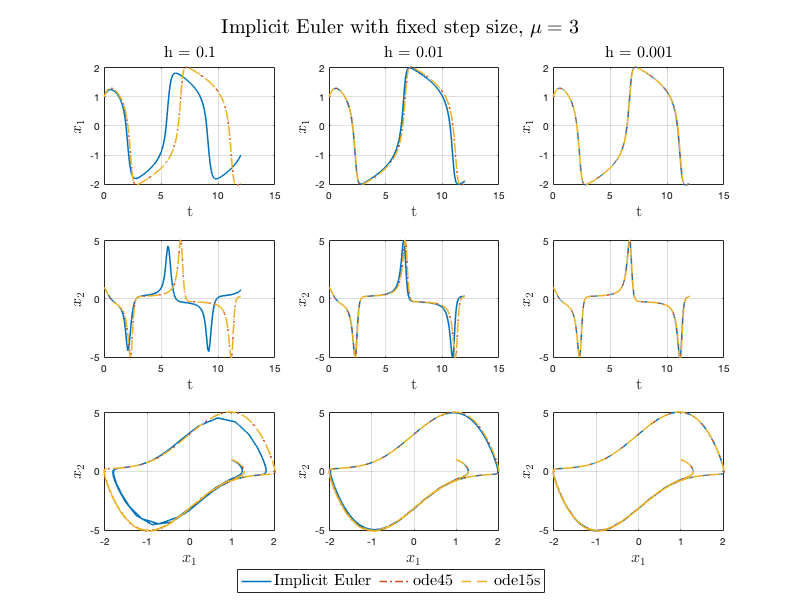
\includegraphics[width=\textwidth]{graphics/opg3/mu3_fixed.png}
    \caption{Solution to Van der Pol with $\mu = 3$ using fixed step sizes}
    \label{fig3:fixed_mu3}
\end{figure}

Table \ref{tab3:mu3_fixed} shows the CPU time and number of function evaluations when solving the Van der Pol problem with $\mu = 3$ using different time steps and Matlab ODE solvers. Notice that with $h=0.1$ the implicit Euler is much faster and uses less function evaluations that any of the other methods, however, as seen above the results are also quite poor. A time step of $h=0.01$ yields similar run time to ODE15s---but with a slight deviation in the results. A step size of $h=0.001$ is by far the slowest of the methods, and the one that uses the most function evaluations. One of the reasons why ODE45 and ODE15s are able to outperform the implicit Euler with fixed step size is because they are able to adjust the step size such that a larger step size is used in the parts with a slower dynamic and vice versa. 

Notice that ODE45 seems to outperform ODE15s. This is a good indication that the problem is not particular stiff, i.e., it is not worth while to use an implicit method that comes with additional computational cost. 

\begin{table}[H]
    \centering
    \caption{CPU time and function evaluations of implicit Euler with fixed time step and Matlab ODE solvers}
    \begin{tabular}{|c||c|c|c|c|c|c|} \hline
         \textbf{Method}    & $h=0.1$&   $h=0.01$ & $h=0.001$ & ODE45 & ODE15s     \\ \hline \hline 
         \textbf{Time}      & 0.0061 &   0.0162  &   0.0962 & 0.0046 & 0.0175   \\ \hline
         \textbf{Fun evals} & 807   &     5421   & 48001 & 1069 & 926  \\ \hline
    \end{tabular}
    \label{tab3:mu3_fixed}
\end{table}



Figure \ref{fig3:adap_mu3} shows the numerical solution to the Van der Pol problem with $\mu = 3$ for implicit Euler with adaptive time steps and $AbsTol=RelTol \in \{10^{-2}, 10^{-4}, 10^{-6}\}$, ODE45 and ODE15s. Notice also that for $Tol = 10^{-2}$ there is a quite big difference between the implicit Euler solution and the other solutions; for $Tol = 10^{-4}$ the difference is almost not visible and for $Tol = 10^{-6}$ there is no visible difference anymore.

\begin{figure}[H]
    \centering
    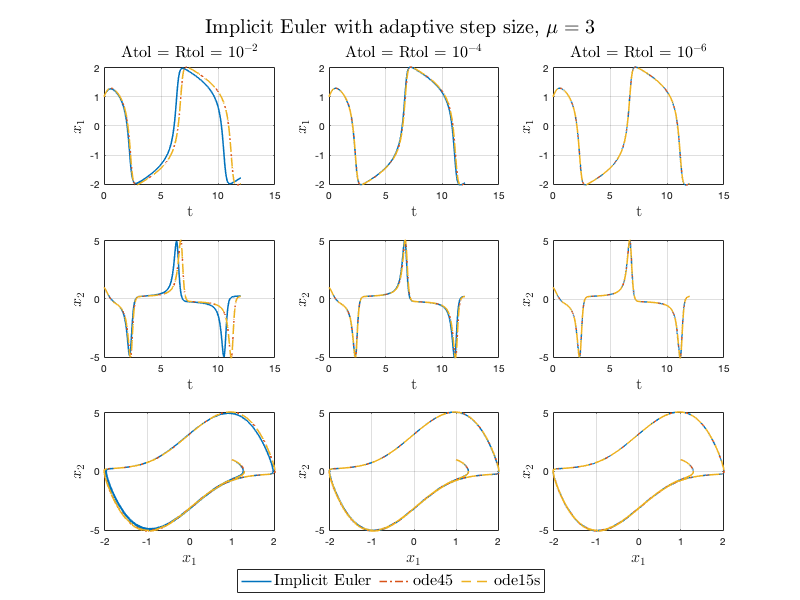
\includegraphics[width=\textwidth]{graphics/opg3/mu3_adap.png}
    \caption{Solution to Van der Pol with $\mu = 3$ using adaptive step sizes}
    \label{fig3:adap_mu3}
\end{figure}

Table \ref{tab3:mu3_adap} shows that CPU time and number of function evaluations when solving the Van der Pol problem with $\mu = 3$ using different tolerances and Matlab ODE solvers. Notice that with $Tol = 10^{-2}$ the implicit Euler is relatively fast (slower than ODE45 but faster than ODE15s), however, as seen above the results are also quite poor. Using $Tol = 10^{-4}$ yields higher run time than ODE15s, but with very little deviation in the results. Finally $Tol = 10^{-6}$ is by far the slowest of the methods, and the one that uses the most function evaluations. One of the reasons why ODE45 and ODE15s are able to outperform the implicit Euler with adaptive step size is because they are higher order methods. This means that they are able to take larger step sizes, which requires less time.

\begin{table}[H]
    \centering
    \caption{CPU time and function evaluations of implicit Euler with adaptive time step and Matlab ODE solvers}
    \begin{tabular}{|c||c|c|c|c|c|c|} \hline
         \textbf{Method}    & $Tol = 10^{-2}$&   $Tol = 10^{-4}$ & $Tol = 10^{-6}$ & ODE45 & ODE15s     \\ \hline \hline 
         \textbf{Time}      & 0.0127  &  0.0845  &  0.4249 & 0.0046 & 0.0175   \\ \hline
         \textbf{Fun evals} & 3575   &     16851    &   166983 & 1069 & 926  \\ \hline
    \end{tabular}
    \label{tab3:mu3_adap}
\end{table}

Figure \ref{fig3:adap_mu3_h} shows the used step sizes for the different tolerances. The red crosses mark whenever the step size controller failed to set the step size correctly, i.e., whenever the estimated (using step doubling) error was larger than the allowed maximum. Notice that the behaviour of all three tolerances are quite similar. Also notice that the step sizes vary by almost a factor 100! This means that even though the problem is not very stiff, there still is enough change in dynamics that the optimal step size vary by a factor 100. 

\begin{figure}[H]
    \centering
    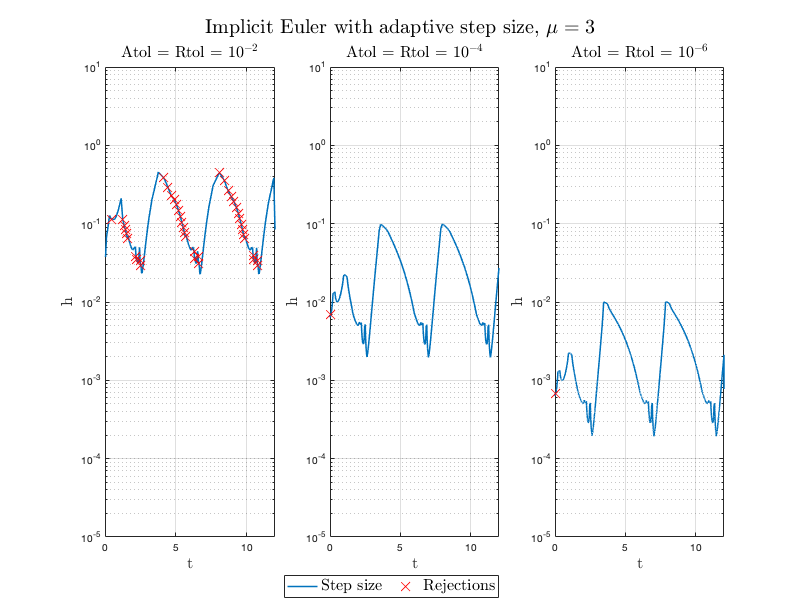
\includegraphics[width=\textwidth]{graphics/opg3/mu3_h.png}
    \caption{Step sizes when solving the Van der Pol with $\mu = 3$ at different tolerances}
    \label{fig3:adap_mu3_h}
\end{figure}

\subsection{Van der Pol, $\mu = 20$}
The Van der Pol problem with $\mu = 20$ is a more complicated problem. The dynamics of the problem is largely defined by the $\mu$ parameter. In particular, the problem becomes more stiff when $\mu$ is increased.

Figure \ref{fig3:fixed_mu20} shows the numerical solution to the Van der Pol problem with $\mu = 3$ for implicit Euler with $h \in \{0.1, 0.01, 0.001\}$, ODE45 and ODE15s. Notice that there is no visible difference between the solution obtained by ODE45 and ODE15s. For $h=0.1$ the solution does not diverge (as the explicit Euler did), however, it deviate substantially from the other solutions! There is a quite big difference between the implicit Euler solution and the other solutions for $h=0.01$. The difference is smaller for $h=0.001$, but it is still visible. This hints that it is a bad idea to use a step size larger than $h=0.001$ for this particular problem, and in fact we should use an even lower step size.

Notice that for the explicit Euler, we saw that the errors came because the curve was "behind" the rest, i.e., the sudden change in value for $x_1$ or $x_2$ came too late. Now we see the exact opposite---the sudden spikes comes too early. This is a key difference between the left point and right point method, i.e., explicit- and implicit Euler. The implicit Euler has much better convergence properties, which is also why we do not see any of the solutions diverge, albeit with some large errors. 

\begin{figure}[H]
    \centering
    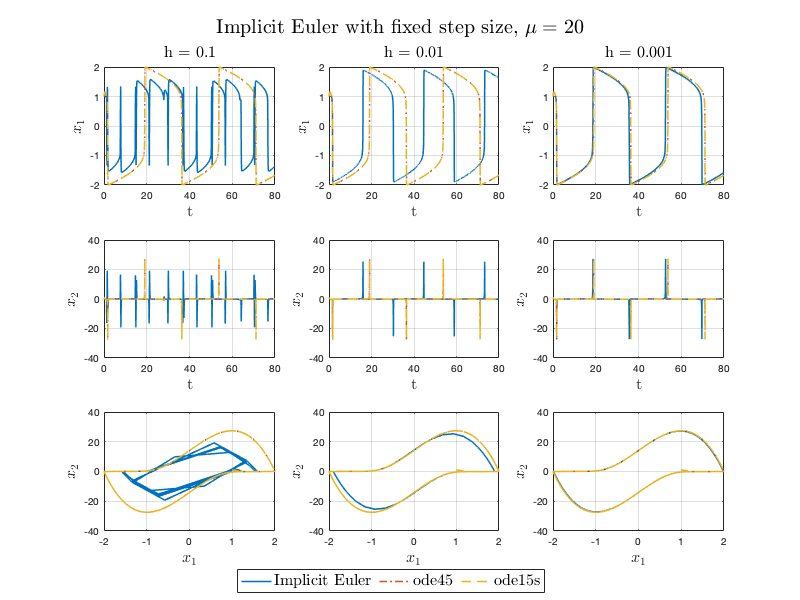
\includegraphics[width=\textwidth]{graphics/opg3/mu20_fixed.png}
    \caption{Solution to Van der Pol with $\mu = 20$ using fixed step sizes}
    \label{fig3:fixed_mu20}
\end{figure}

Table \ref{tab3:mu20_fixed} shows that CPU time and number of function evaluations when solving the Van der Pol problem with $\mu = 20$ using different time steps and Matlab ODE solvers. Notice that with $h=0.1$ the implicit Euler is as fast as any of the other methods, however, as seen above the results are also completely wrong. A time step of $h=0.01$ yields similar run time to ODE15s---but with substantial deviations in the results. A step size of $h=0.001$ is by far the slowest of the methods, and the one that uses the most function evaluations. One of the reasons why ODE45 and ODE15s are able to outperform the implicit Euler with fixed step size is because they are able to adjust the step size such that a larger step size is used in the parts with a slower dynamic and vice versa. 

Notice that ODE45 does not outperform ODE15s anymore. This is a good indication that the problem is stiff, i.e., it is worth while to use an implicit method that even when it comes with additional computational cost. The implicit method is also able to use far less function evaluations than the DoPri54. 

\begin{table}[H]
    \centering
    \caption{CPU time and function evaluations of implicit Euler with fixed time step and Matlab ODE solvers}
    \begin{tabular}{|c||c|c|c|c|c|c|} \hline
         \textbf{Method}    & $h=0.1$&   $h=0.01$ & $h=0.001$ & ODE45 & ODE15s     \\ \hline \hline 
         \textbf{Time}      & 0.0325  &  0.0691  &  0.3027 & 0.0370 & 0.0504   \\ \hline
         \textbf{Fun evals} & 7001    &   33175   &   199129 & 8461 & 926  \\ \hline
    \end{tabular}
    \label{tab3:mu20_fixed}
\end{table}



Figure \ref{fig3:adap_mu20} shows the numerical solution to the Van der Pol problem with $\mu = 20$ for implicit Euler with adaptive time steps and $AbsTol=RelTol \in \{10^{-2}, 10^{-4}, 10^{-6}\}$, ODE45 and ODE15s. Notice also that for $Tol = 10^{-2}$ there is a quite big difference between the implicit Euler solution and the other solutions; for $Tol = 10^{-4}$ the difference is almost not visible and for $Tol = 10^{-6}$ there is no visible difference anymore.

\begin{figure}[H]
    \centering
    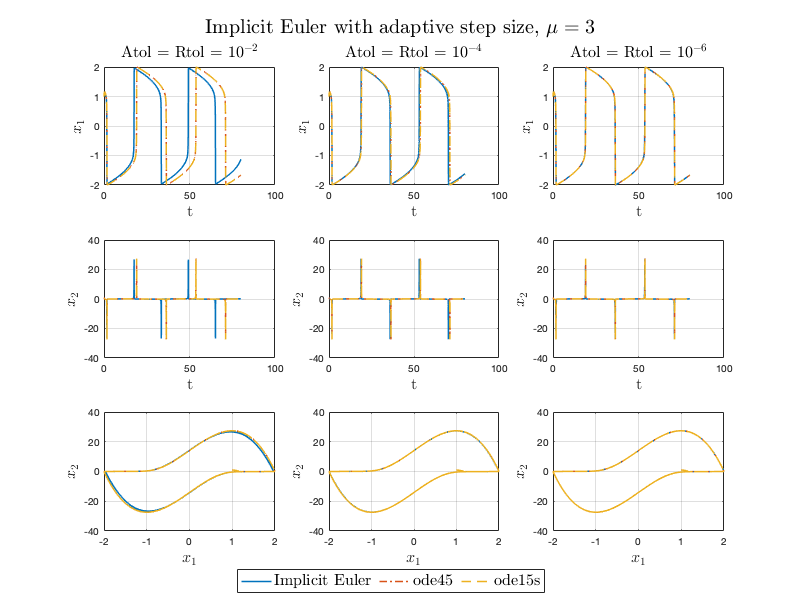
\includegraphics[width=\textwidth]{graphics/opg3/mu20_adap.png}
    \caption{Solution to Van der Pol with $\mu = 20$ using adaptive step sizes}
    \label{fig3:adap_mu20}
\end{figure}

Table \ref{tab3:mu20_adap} shows that CPU time and number of function evaluations when solving the Van der Pol problem with $\mu = 20$ using different tolerances and Matlab ODE solvers. Notice that with $Tol = 10^{-2}$ the implicit Euler is already slower than Matlab ODE solvers, and as seen above the results also deviate from the rest. Using $Tol = 10^{-4}$ yields even higher run time, but now with very little deviation in the results. Finally $Tol = 10^{-6}$ is by far the slowest of the methods, and the one that uses the most function evaluations (by a quite substantial amount). 

One of the reasons why ODE45 and ODE15s are able to outperform the implicit Euler with adaptive step size is because they are higher order methods and because they are implemented very very efficiently. 

\begin{table}[H]
    \centering
    \caption{CPU time and function evaluations of implicit Euler with adaptive time step and Matlab ODE solvers}
    \begin{tabular}{|c||c|c|c|c|c|c|} \hline
         \textbf{Method}    & $Tol = 10^{-2}$&   $Tol = 10^{-4}$ & $Tol = 10^{-6}$ & ODE45 & ODE15s     \\ \hline \hline 
         \textbf{Time}      & 0.1045 &    0.4818 &    0.8793 & 0.0386 & 0.0612   \\ \hline
         \textbf{Fun evals} &  21977 &  46903 &      446091 & 8461 & 2944  \\ \hline
    \end{tabular}
    \label{tab3:mu20_adap}
\end{table}

Figure \ref{fig3:adap_mu20_h} shows the used step sizes for the different tolerances. The red crosses mark whenever the step size controller failed to set the step size correctly, i.e., whenever the estimated (using step doubling) error was larger than the allowed maximum. Notice that the behaviour of all three tolerances are quite similar. Also notice that the step sizes vary by more than a factor 1000! This is a good indication that the problem is stiff. Also notice that for $AbsTol=RelTol=10^{-2}$ the step size controller fails at setting the correct step size many times. This again indicates that there is a rapid change in dynamics, which leads to a large needed change in step size---larger than anticipated by the step size controller.

\begin{figure}[H]
    \centering
    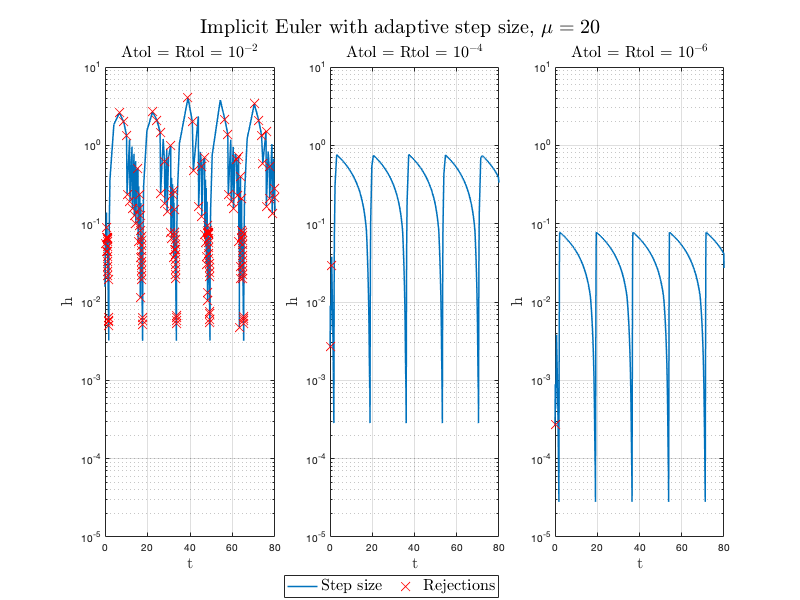
\includegraphics[width=\textwidth]{graphics/opg3/mu20_h.png}
    \caption{Step sizes when solving the Van der Pol with $\mu = 20$ at different tolerances}
    \label{fig3:adap_mu20_h}
\end{figure}






